\documentclass{iopconfser}

\usepackage{graphicx}
\usepackage{amsmath,amssymb}
\usepackage[separate-uncertainty=true]{siunitx}
\usepackage{booktabs}
\usepackage{hyperref}
\usepackage{soul}
\graphicspath{{figures/}}

\begin{document}

\title{Gamma detection for source localisation in targeted alpha therapy}

\author{C. De Sio$^{1}$, L. Abu Sabah$^{1}$, J. Duan$^{1}$, Y. Shi$^{1}$,
S. Williams$^{1}$ and J. Velthuis$^{1}$}

\affil{$^1$School of Physics, University of Bristol, Bristol, United Kingdom}

\begin{abstract}
Targeted alpha therapies can deliver a highly localised dose to tumour sites, but treatment
planning and effectiveness depend on whether the radionuclide source remains near
the intended site after administration. In the AlphaGlue delivery concept~\cite{AlphaGlue2025},
alpha emitters are applied to a tumour region in a thin glue layer. We present
a Geant4 simulation study showing that decay-chain gamma detection can
distinguish retained, broadly diffused and locally displaced source states in
an AlphaGlue-like geometry. Using Geant4, 50 repeated simulations of 10,000 primary events were generated, and
baseline-subtracted gamma-hit profiles were successfully used to reconstruct the broad diffusion
fraction with $R^2=0.9987$ and a mean absolute error of about one percentage
point. Localised-source residuals identified displaced activity with mean
position errors of 16--30 mm. These results support gamma detection as a
candidate method for emitter-position monitoring, treatment planning and
delivery verification.
\end{abstract}

\section{Introduction}

In targeted alpha therapy, the delivered dose is strongly local. A treatment
plan therefore depends not only on the initial activity distribution, but also
on whether source material and progeny remain near the intended deposition
site, diffuse into surrounding tissue or are redistributed by biological
transport~\cite{laura,heger}. The
\href{https://doi.org/10.3390/biomedinformatics5040058}{AlphaGlue concept}
proposes suspending alpha emitters in a thin glue layer applied to tissue
\cite{AlphaGlue2025}. The concept has previously been evaluated with Geant4
and Geant4-DNA simulations for dose and DNA-damage modelling
\cite{Geant4,Geant4DNA}. This study investigates whether the accompanying
gamma signal can be used as a theranostic observable to monitor emitter
position, detect source movement and provide useful information as a function
of detection time.

\section{Simulation model}

Photon transport was simulated with the Geant4 toolkit~\cite{Geant4}. The
model places a \(\SI{40}{mm} \times \SI{2}{mm} \times \SI{40}{mm}\) loaded
glue layer on the \(+y\) surface of a
\(\SI{20}{cm} \times \SI{20}{cm} \times \SI{150}{cm}\) water phantom. Six
detector panels surround the phantom at \(\SI{20}{cm}\) from the water
surface. Each photon entry into a detector panel is counted as one hit.

Seven source configurations were studied to separate three clinically
relevant possibilities: emitter retained in the loaded glue layer, emitter
broadly mixed into the surrounding volume and emitter transported to a
localised displaced region. The retained-source case is used as the baseline.
Some alpha emitters in the decay chain can be taken up by the blood, with large
variation reported between experiments~\cite{laura,heger}. This further
emphasises the need for local dose verification. The simulations therefore
include cases in which 10\%, 50\% or 90\% of the radioisotope is distributed
throughout the water volume, and cases in which 20\%, 40\% or 60\% of the
source is placed in a small displaced water region.
The geometry is described in Fig.~\ref{fig:geometry}, along with example detector displays showing the three clinical scenarios.
Each configuration was simulated with 50 independent repetitions of 10,000
primary decays, giving 500,000 simulated decays per configuration and
3.5 million simulated decays across all source states. The repeated runs
define the run-to-run uncertainty used in the residual and detectability
analysis. The simulated decays
are rescaled to a DaRT-like reference activity of
\(3~\mu\mathrm{Ci}\) (\(\SI{111}{\kilo\becquerel}\)), matching the order
of a single DaRT seed~\cite{dart}.

\begin{figure}[htbp]
\centering
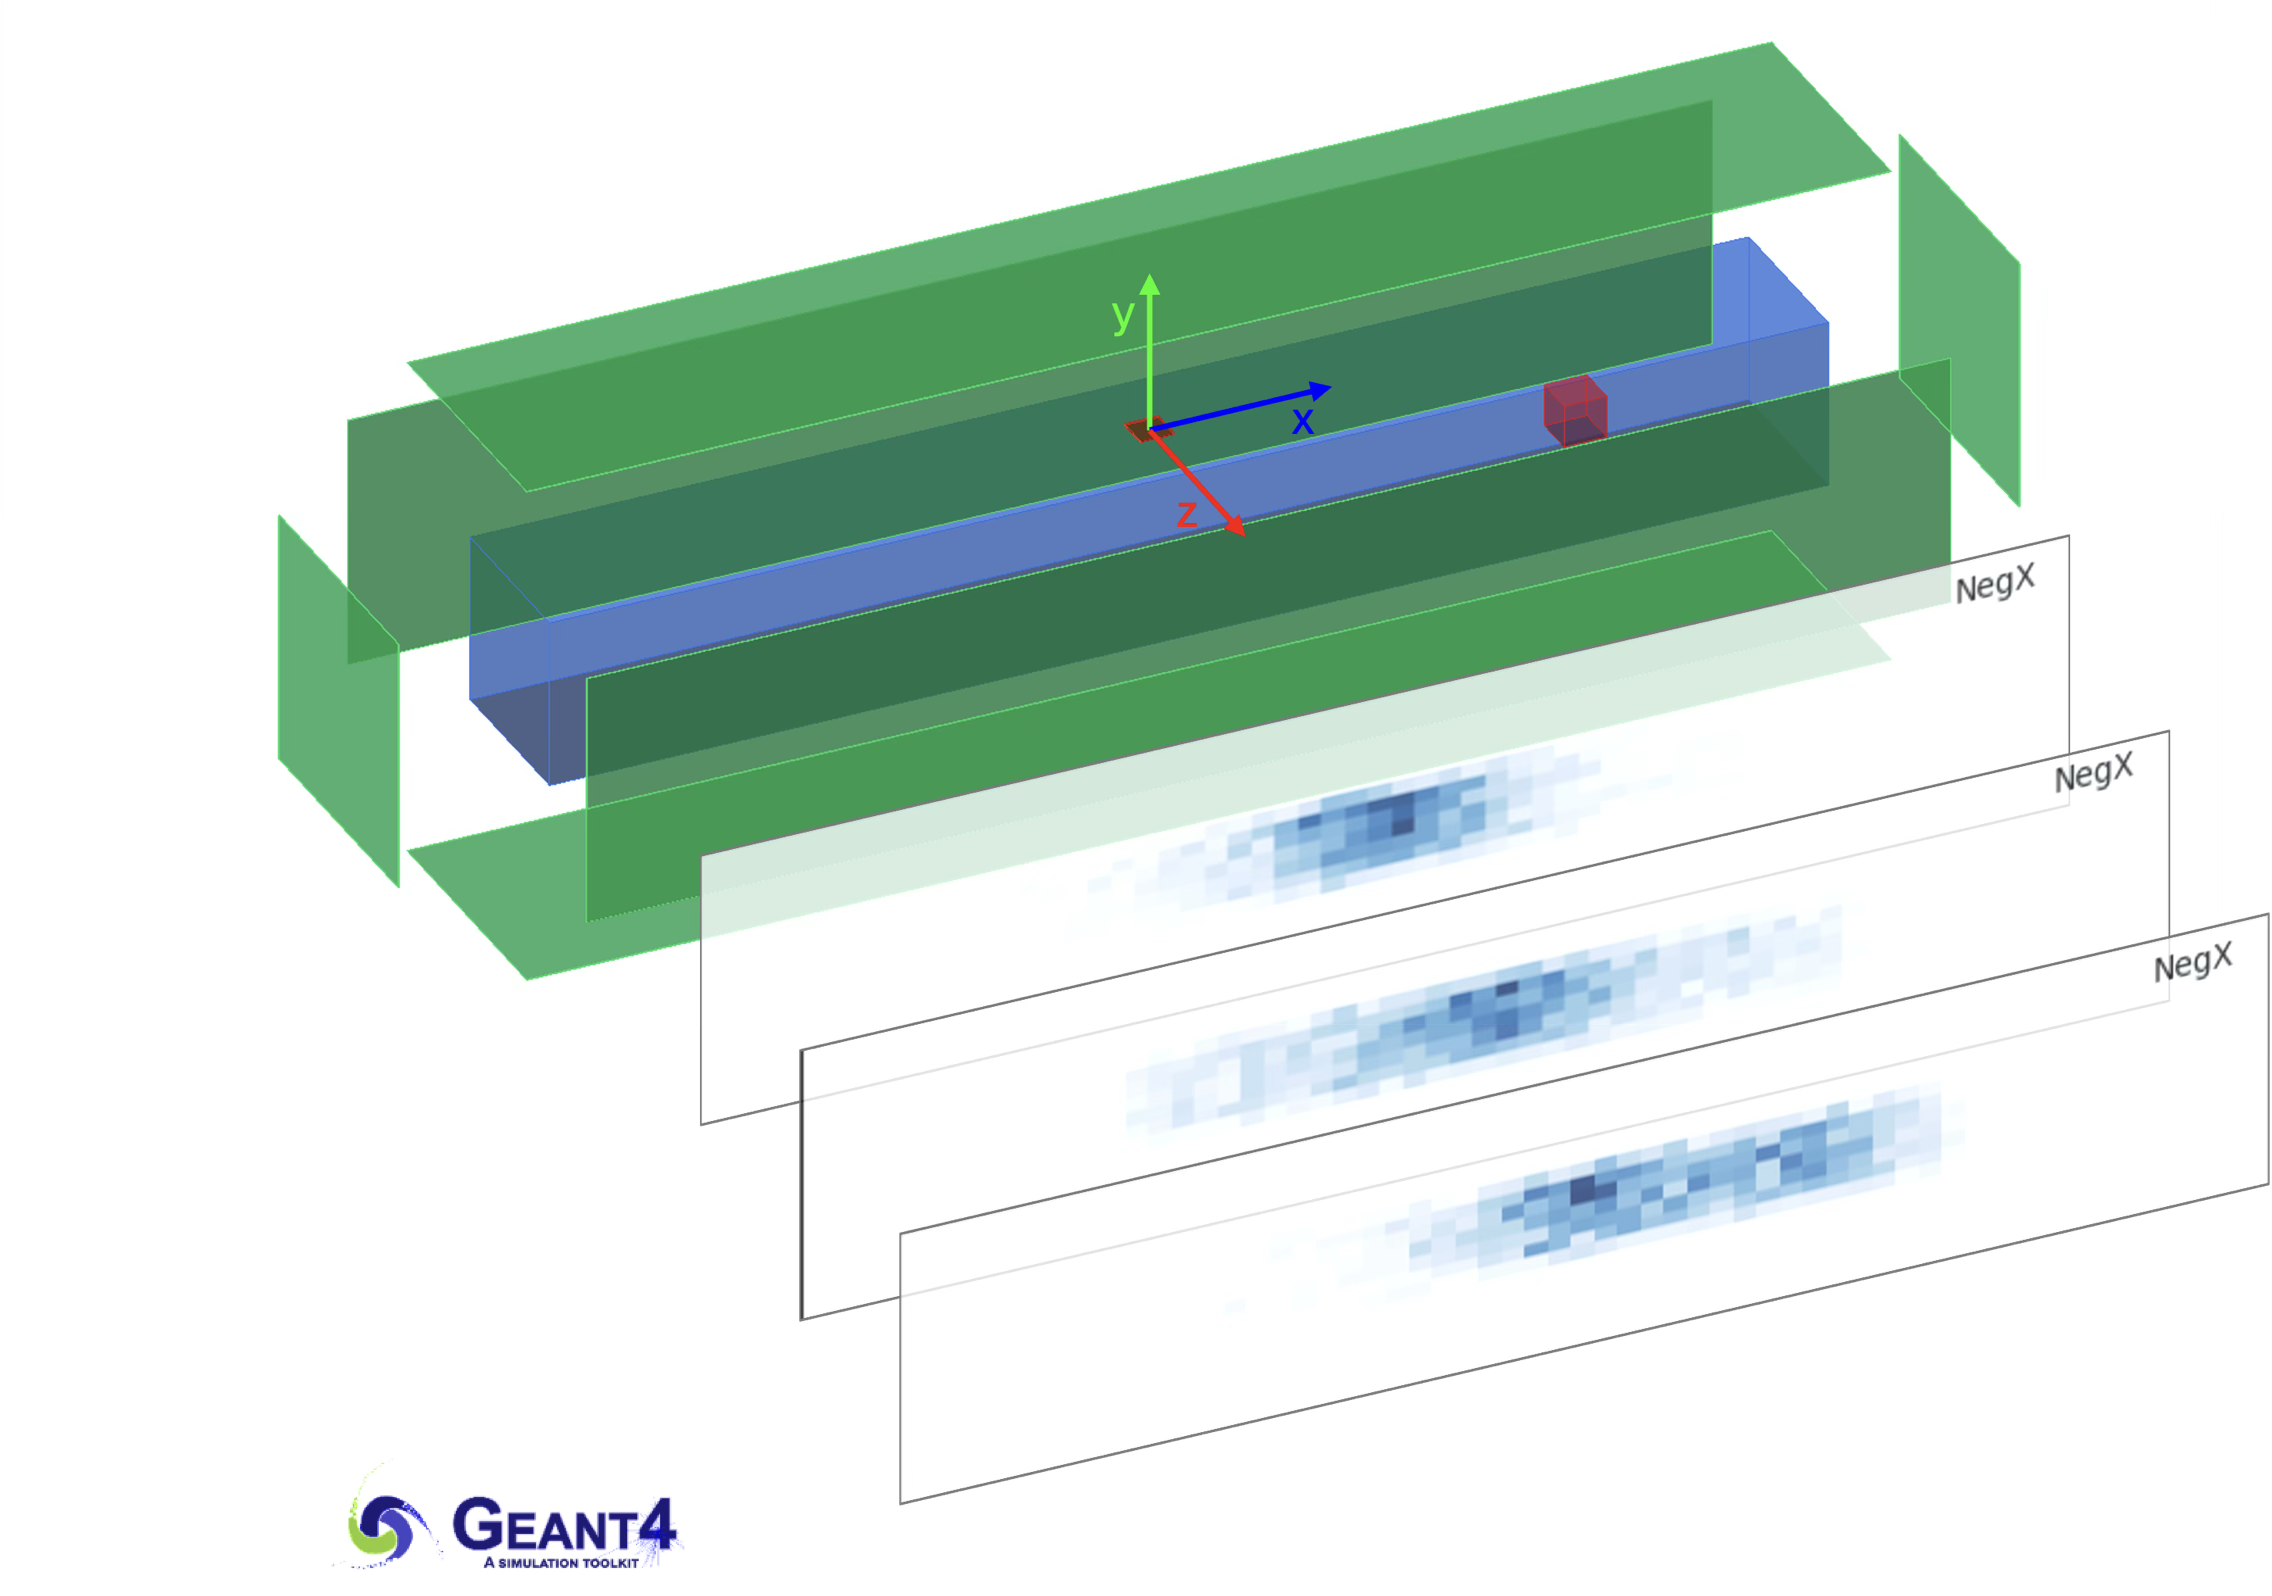
\includegraphics[width=0.72\linewidth]{aocmp_poster_geometry.png}
\caption{Simulation geometry showing the water phantom (blue), surrounding
detector panels (green), a displaced source (red) and example detector
projections for baseline (inner-most), broad redistribution (middle), displaced localisation (outer-most).}
\label{fig:geometry}
\end{figure}

\section{Baseline subtraction}

The total detector-entry rate changed only weakly between retained and
redistributed source states. Between the retained
baseline and the 90\% broad-diffusion case, the difference in hit count changed only by 3.8\%. In contrast,
baseline-subtracted profiles show a clear spatial signature. The retained
source defines the reference profile \(\bar{h}^{B}_{p}(z)\) for detector panel
\(p\). Candidate source states are represented by
\begin{equation}
\Delta h_p(z)=h_p(z)-\bar{h}^{B}_{p}(z),
\end{equation}
with the repeated baseline simulations defining the bin-wise noise scale.
Positive residuals mark detector regions where the candidate produces more
gamma entries than the retained-source case, while negative residuals mark
depleted regions. Broad diffusion widens the residual pattern and changes the
balance between the glue-facing and opposite detector panels. Localised
displacement produces a shifted excess near the displaced source region.

\begin{figure}[htbp]
\centering
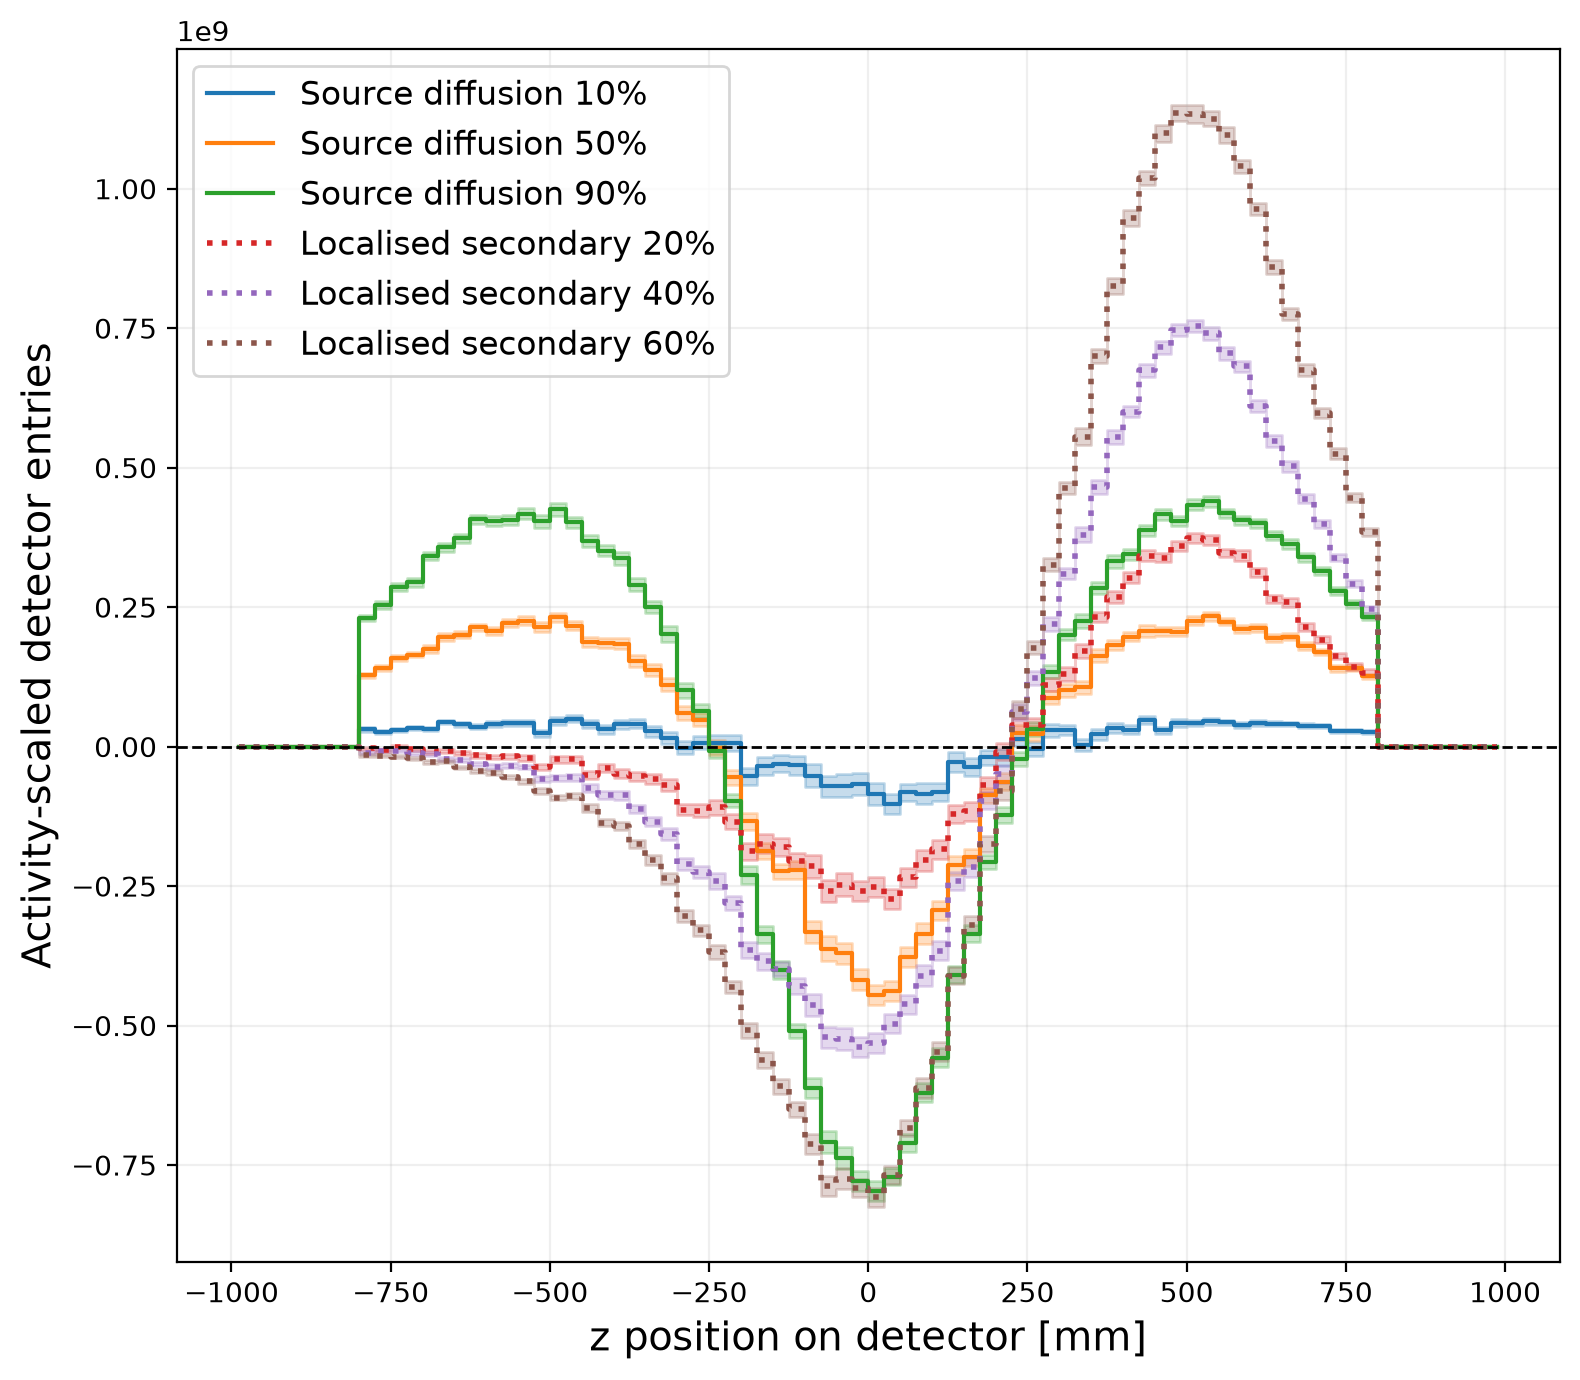
\includegraphics[width=0.60\linewidth]{poster_01_baseline_subtracted_profiles_xsum_all_cases.png}
\caption{Activity-normalised, baseline-subtracted combined\(+x\) and \(-x\) detector
profiles for broad diffusion and localised displacement. Shaded bands show
variation across repetitions.}
\label{fig:residual_profiles}
\end{figure}

Figure~\ref{fig:residual_profiles} shows that baseline-subtracted spatial hit patterns is a good indicator of source movement.

\section{Signal analysis and source redistribution metrics}

The residual analysis was organised into three source-monitoring metrics.
First, diffusion percentage was inferred from profile-shape features \hl{and panel-balance
changes}. The response of the \(+y\) panel decreases as activity moves away from the
glue layer, while the width of the profile and the share of the side-panels increase. Second,
activity-retention observables used the central \(+y\) region of interest
(ROI) as an applicator-facing signal. \hl{This estimates activity still consistent
with the retained-source geometry, but is interpreted only after a
secondary-source test because compact displaced activity can also suppress
the central signal.} Third, compact secondary sources were searched for using
positive residuals in a displaced-region ROI and panel-asymmetry changes that
\hl{are small for broad diffusion but large for off-applicator localisation}.

\begin{figure}[htbp]
\centering
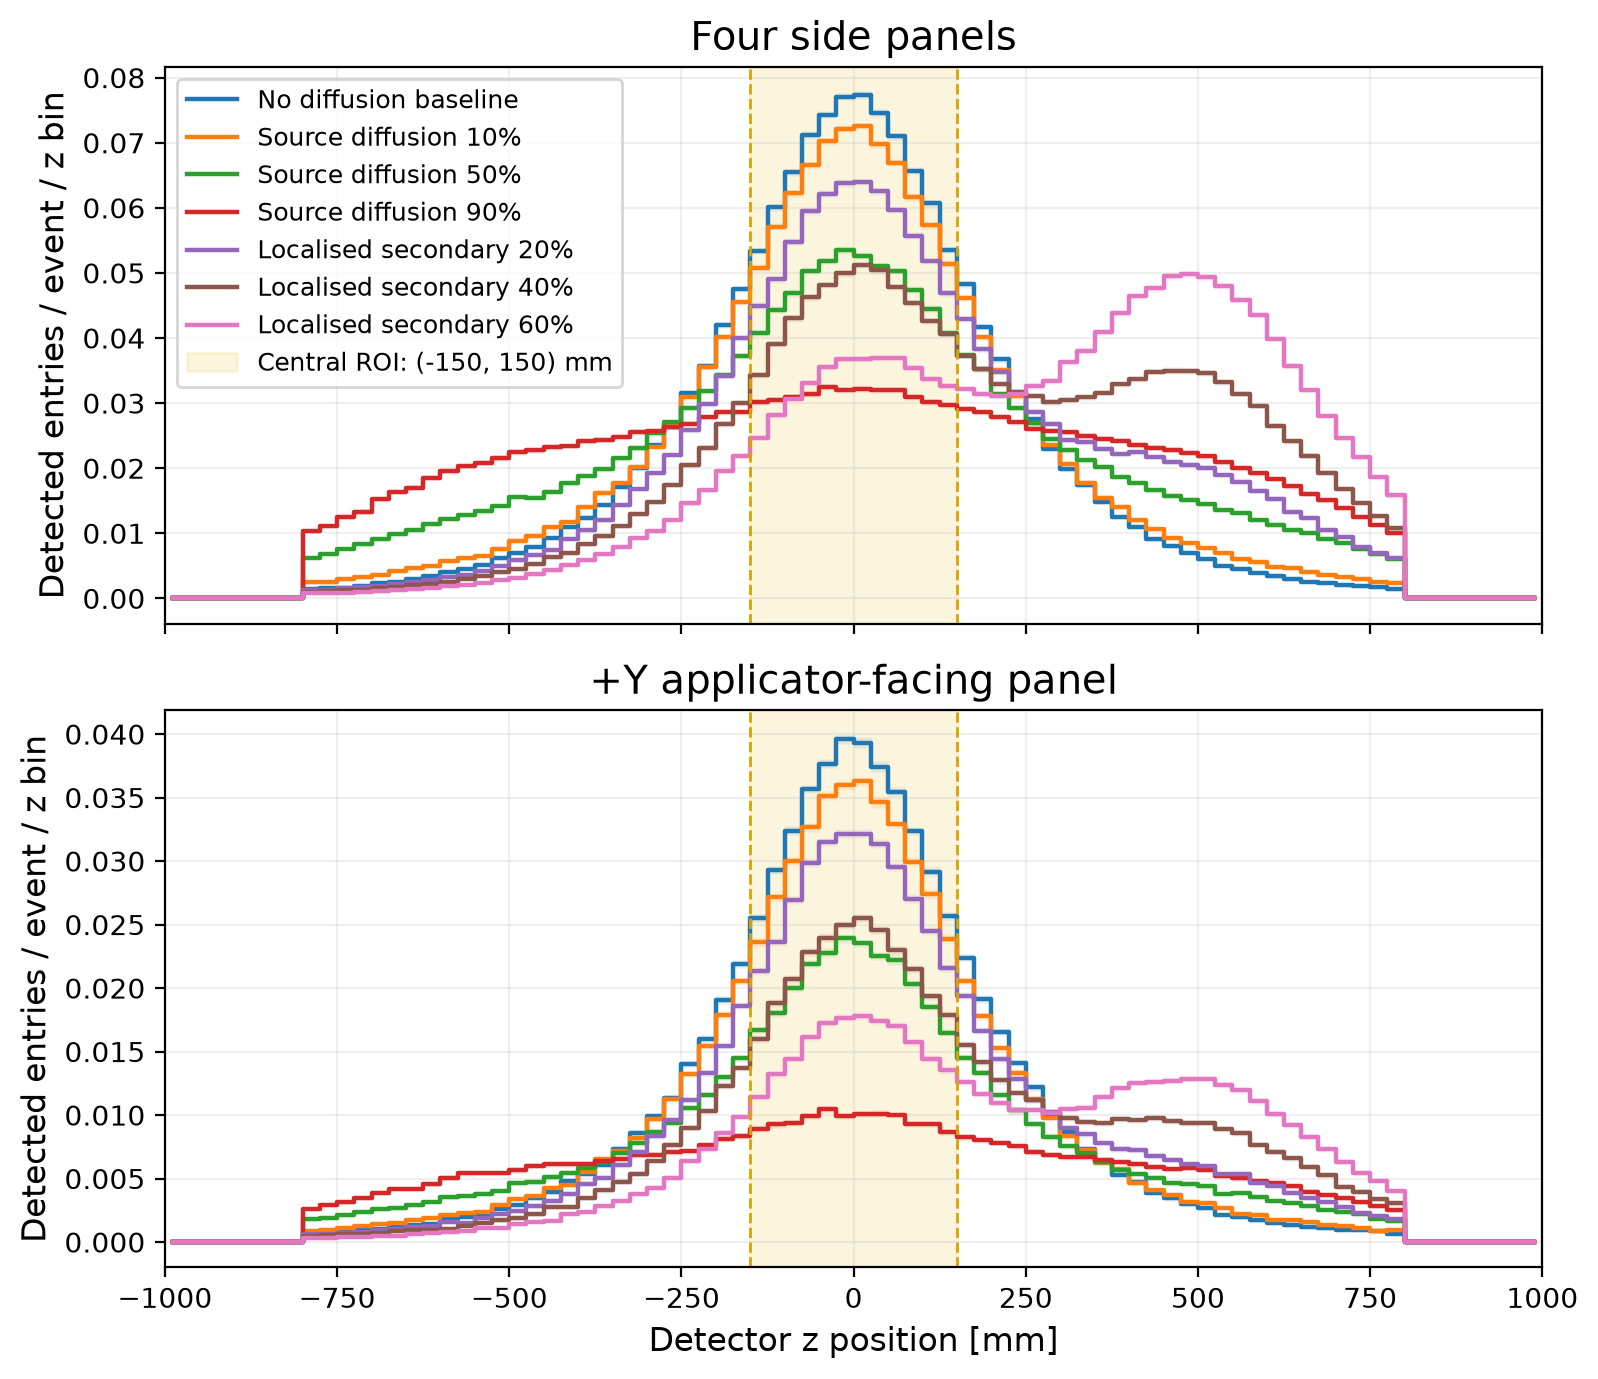
\includegraphics[width=0.75\linewidth]{material_signal_central_roi_profiles.png}
\caption{Central-ROI signal used to separate retained applicator response
from activity redistributed outside the applicator region.}
\label{fig:central_roi}
\end{figure}

\begin{figure}[htbp]
\centering
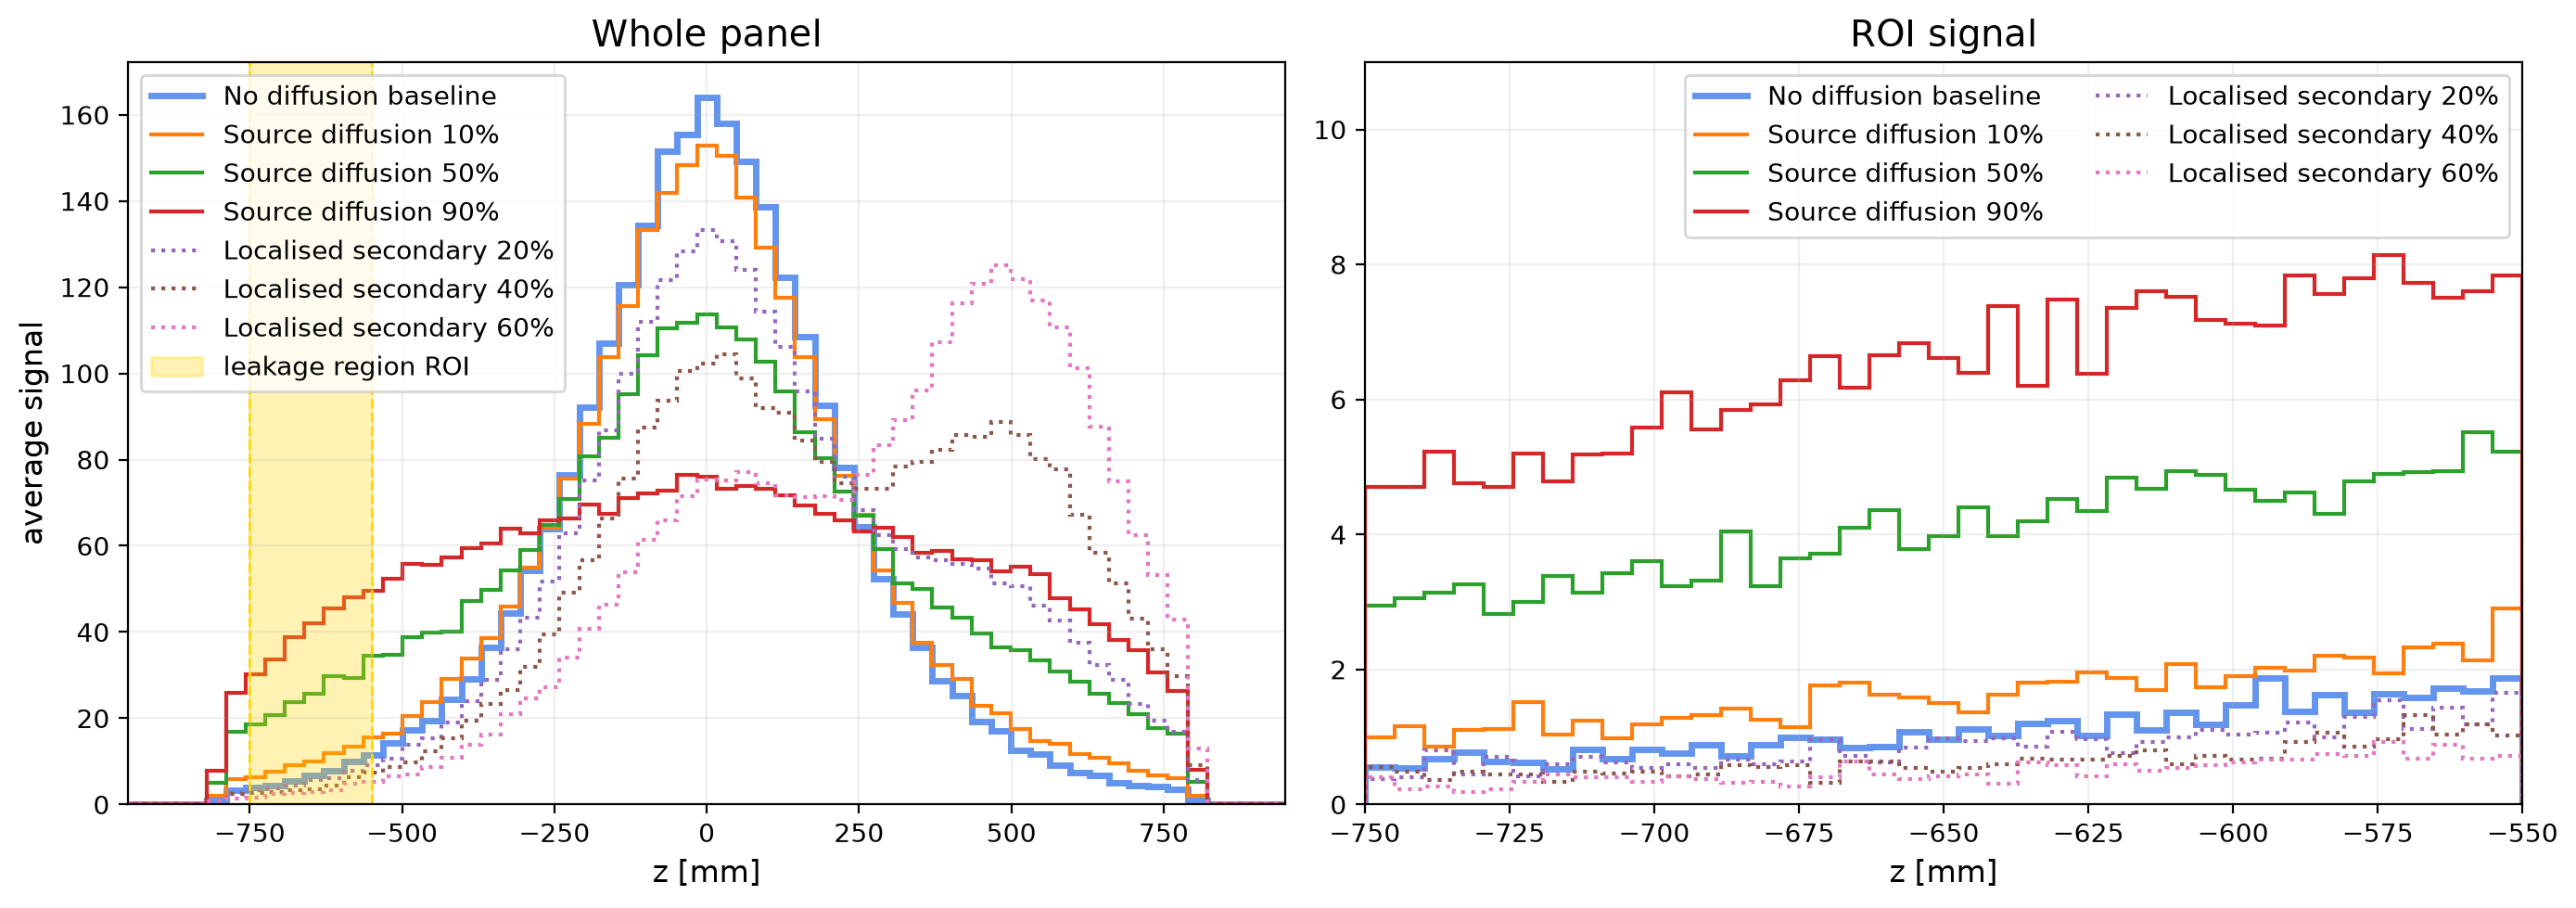
\includegraphics[width=0.98\linewidth]{poster_03c_leakage_roi_side_by_side.png}
\caption{Whole \(x\)-panel profiles (left) and the displaced-region ROI
signal (right). The ROI highlights the broad-diffusion excess outside the
retained-source region.}
\label{fig:leakage_roi}
\end{figure}

For the present geometry, the displaced-source search ROI is centred on the
positive-\(z\) region containing the simulated compact water source. The
secondary-source score integrates the positive residual in this ROI and
compares it with the retained-source baseline variation. If this test is
positive, the location is estimated from the positive-residual centroid on
the detector views that best project the source onto the longitudinal axis.
Diffusion fraction is reported for broad redistribution candidates, while
localised cases are first reported as compact secondary-source detections with
an estimated position. \hl{The leakage comparison is shown in }Fig.~\ref{fig:leakage_roi}.

\section{Results}

\subsection{Signal inference}

Using profile-shape features from repeated simulations, the broad diffusion
fraction was recovered with \(R^2=0.9987\) and a mean absolute error of about
one percentage point. A separate secondary-source metric identified the
localised displaced source in all 20\%, 40\% and 60\% localised-displacement
cases. The reconstructed displaced-source positions were approximately
\(z=\SI{516}{mm}\), \(\SI{528}{mm}\) and \(\SI{530}{mm}\), respectively,
compared with the simulated \(z=\SI{500}{mm}\) source region. Across these
localised fractions, mean position errors were 16--30 mm.

\begin{figure}[htbp]
\centering
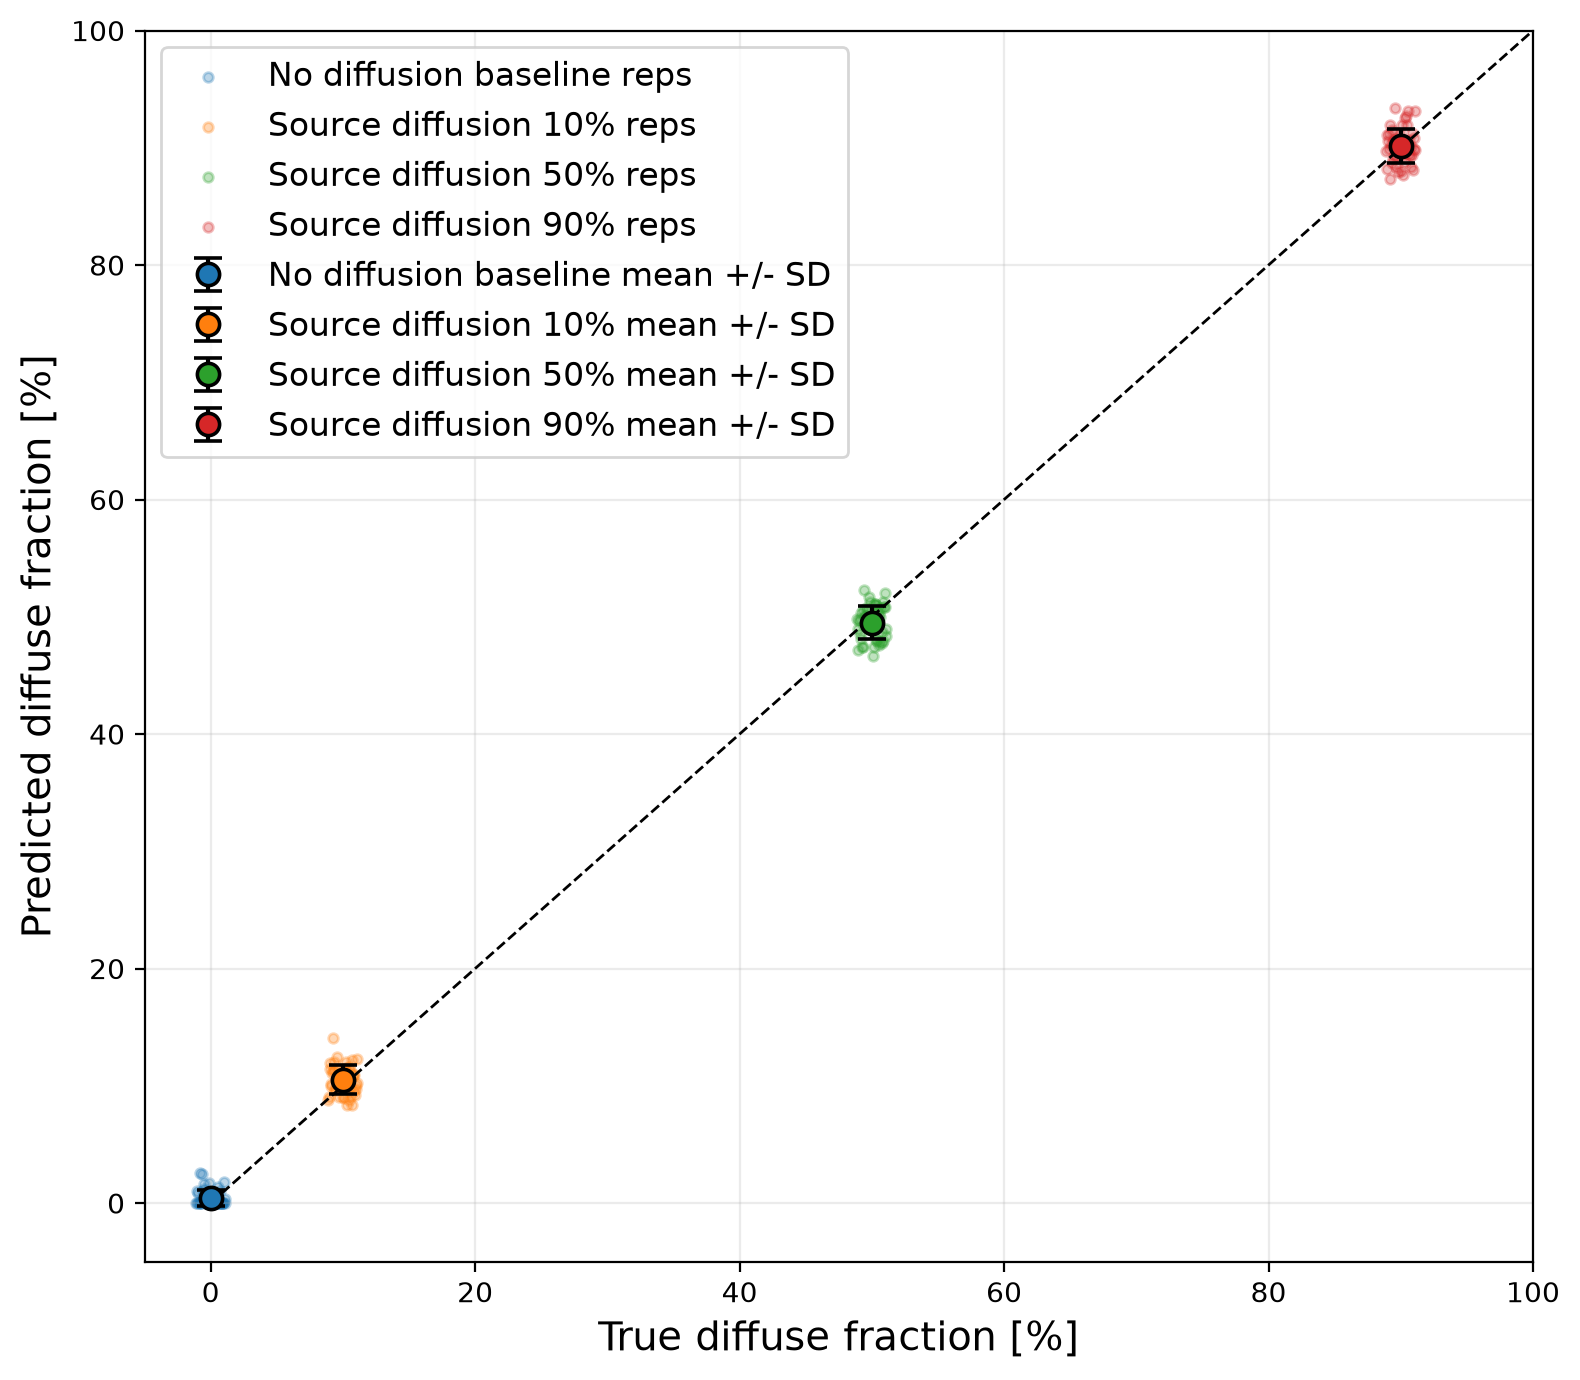
\includegraphics[width=0.5\linewidth]{poster_02_diffusion_fraction_cv_prediction.png}
\caption{Diffusion fraction inferred from 50 independent repetitions. Small
points show individual repetitions and large markers show the mean and
standard deviation.}
\label{fig:diffusion_prediction}
\end{figure}

\begin{figure}[htbp]
\centering
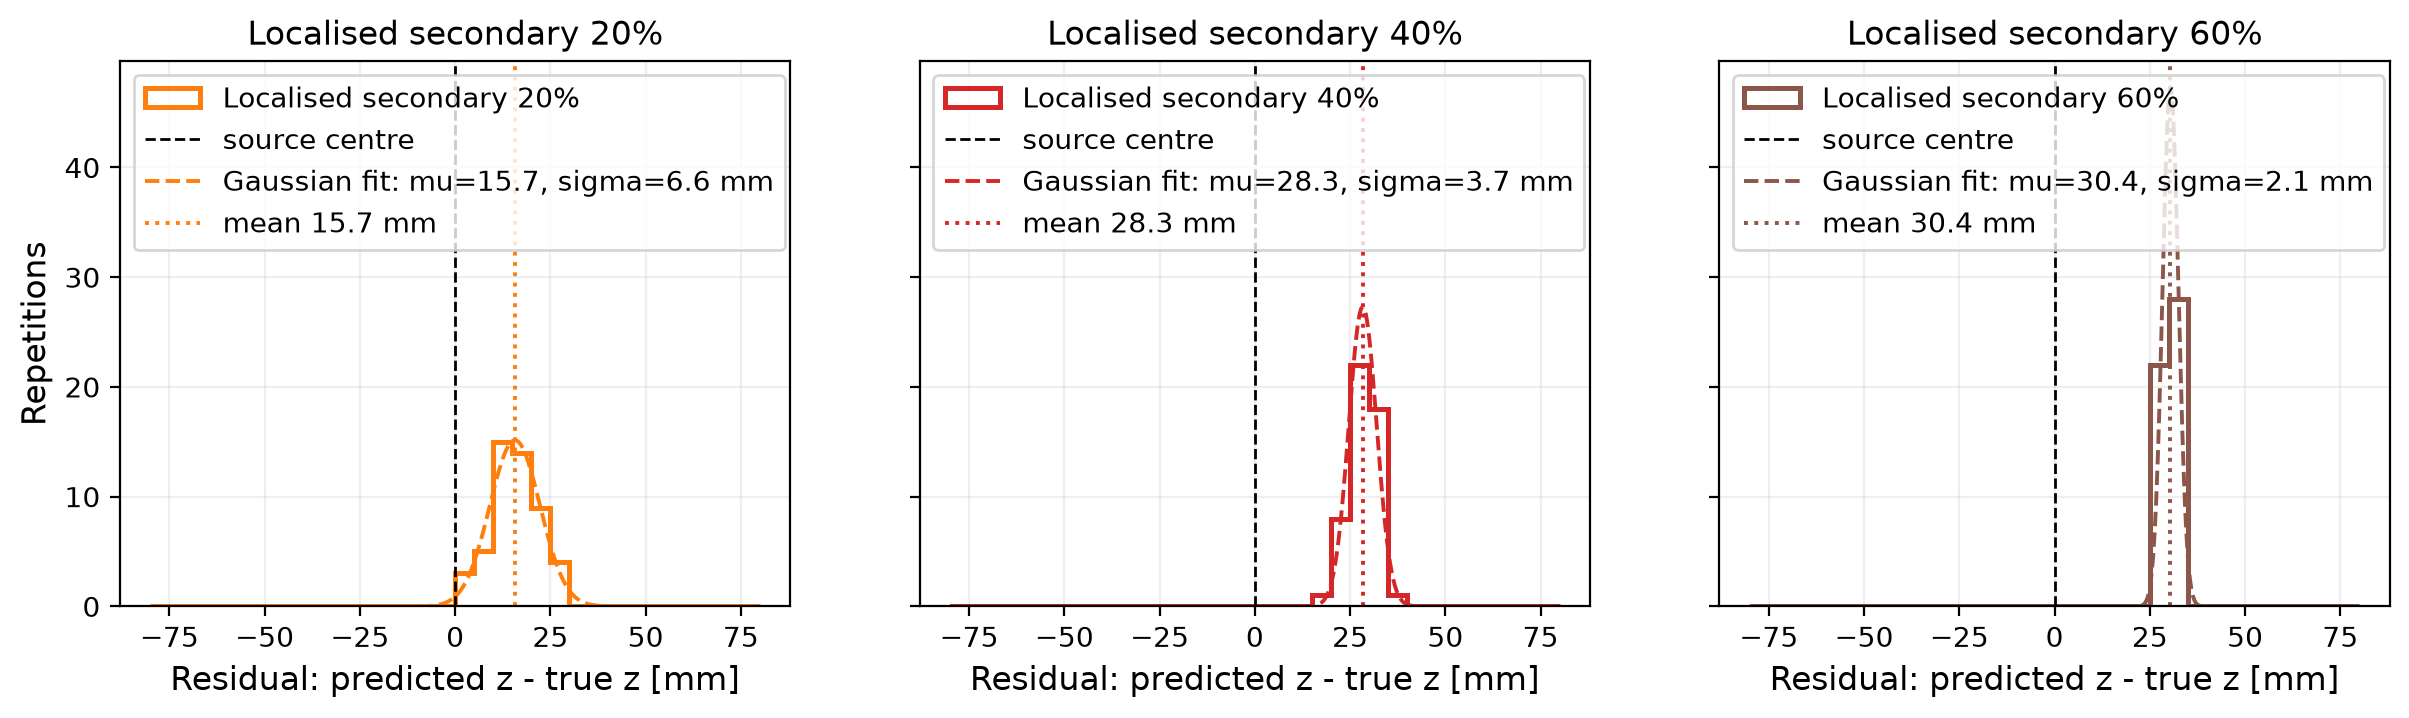
\includegraphics[width=0.98\linewidth]{poster_04b_localised_source_position_residuals.png}
\caption{Localisation residuals across 50 repetitions for each
displaced-source fraction. The dashed black line marks the true source centre;
coloured lines indicate the mean and Gaussian fit.}
\label{fig:source_residuals}
\end{figure}

\subsection{Time dependence}

Cumulative time-window profiles show that the baseline-subtracted signal is
already visible on hour-scale windows and becomes stronger over longer
observation windows. Across the 50 simulation repetitions, detectability was defined as
candidate-baseline separation greater than \(3\sigma\) of the run-to-run
baseline variation. The 50--90\% broad-diffusion and 20--60\%
localised-displacement cases crossed threshold in about 1--2 hours, while the
weaker 10\% broad-diffusion case required about 6 hours. A representative time-window profile is shown in Fig.~\ref{fig:time_windows}. A
\(t<10^6~\mathrm{s}\) analysis cut suppresses a late decay-chain tail while
retaining the early signal relevant to the simulated source-localisation
window.

\begin{table}[htbp]
\centering
\caption{First \(3\sigma\) detection times from the time-window analysis of
50 independent repetitions.}
\label{tab:time_detection}
\begin{tabular}{lc}
\toprule
Case group & First \(3\sigma\) detection \\
\midrule
10\% broad diffusion & about 6 h \\
50--90\% broad diffusion & about 1--2 h \\
20--60\% localised displacement & about 1--2 h \\
\bottomrule
\end{tabular}
\end{table}

\begin{figure}[htbp]
\centering
\begin{minipage}[t]{0.49\linewidth}
\centering
\includegraphics[width=\linewidth]{poster_05_time_window_residual_profiles_loc40.png}
\end{minipage}\hfill
\begin{minipage}[t]{0.49\linewidth}
\centering
\includegraphics[width=\linewidth]{secondary_displaced_roi_zscore_vs_time.png}
\end{minipage}
\caption{Time-dependent residual analysis. Left: cumulative \(+x\) and
\(-x\) profile for 40\% localised displacement, showing a growing excess near
\(z=\SI{500}{mm}\). Right: significance of the distinct displaced-source ROI
signal with observation time.}
\label{fig:time_windows}
\end{figure}

\section{Conclusion}

Decay-chain gamma detection provides source-location information and broad redistribution estimation. Baseline-subtracted profiles distinguish
retained, broadly diffused and locally displaced activity, while residual
features support quantitative estimates of diffusion fraction and displaced
source position. Further work will include detector response, background estimation, and
patient-scale geometries so that activity-normalised profiles can be
interpreted as experimentally measurable count rates.

\begin{thebibliography}{9}

\bibitem{AlphaGlue2025}
Abu Sabah L \textit{et al.} 2025 AlphaGlue: A novel conceptual delivery method
for $\alpha$ therapy \textit{BioMedInformatics} \textbf{5} 58

\bibitem{laura}
Ballisat L \textit{et al.} 2025 Geant4 simulation of the enhanced in-vivo
$^{220}$Rn spread in DaRT \textit{Phys. Med.} \textbf{135} 105005

\bibitem{heger}
Heger G \textit{et al.} 2024 First measurements of radon-220 diffusion in mice
tumors \textit{Med. Phys.} \textbf{51} 5045--5058

\bibitem{Geant4}
Agostinelli S \textit{et al.} 2003 Geant4---a simulation toolkit
\textit{Nucl. Instrum. Methods Phys. Res. A} \textbf{506} 250--303

\bibitem{dart}
Arazi L \textit{et al.} 2010 The treatment of solid tumors by alpha emitters
released from $^{224}$Ra-loaded sources \textit{Phys. Med. Biol.} \textbf{55}
1203

\bibitem{Geant4DNA}
Incerti S \textit{et al.} 2010 The Geant4-DNA project
\textit{Int. J. Model. Simul. Sci. Comput.} \textbf{1} 157--178
\end{thebibliography}

\end{document}
